\begin{figure}[ht]
    \centering
    % First minipage
    \begin{minipage}[b]{0.45\textwidth}
        \centering
        \resizebox{\linewidth}{!}{
            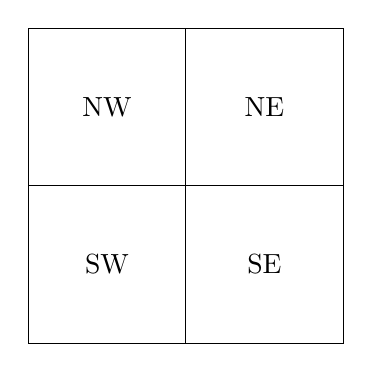
\begin{tikzpicture}
                \draw (1, 1) rectangle (3, 3);
                \draw (1, 3)rectangle (3, 5);
                \draw (3, 1)rectangle (5, 3);
                \draw (3, 3)rectangle (5, 5);
                \node at (2, 2){SW};
                \node at (4, 4){NE};
                \node at (2, 4){NW};
                \node at (4, 2){SE};
            \end{tikzpicture}
        }
        \caption{Квадратная матрица, разделенная на квадранты}
        \label{qmatrix}
    \end{minipage}
    \hfill
    % Second minipage
    \begin{minipage}[b]{0.45\textwidth}
        \centering
        \Tree [.Matrix
                [.NW [] ]
                [.NE [] ]
                [.SW [] ]
                [.SE [] ]
        ]
        \caption{Схематичное изображение одного из узлов дерева квадрантов и его потомков}
        \label{qtree1}
    \end{minipage}
\end{figure}
